%%%%%%%%%%%%%%%%%%%%%%%%%%%%%%%%%%%%%%%%%
% Beamer Presentation
% LaTeX Template
% Version 1.0 (10/11/12)
%
% This template has been downloaded from:
% http://www.LaTeXTemplates.com
%
% License:
% CC BY-NC-SA 3.0 (http://creativecommons.org/licenses/by-nc-sa/3.0/)
%
%%%%%%%%%%%%%%%%%%%%%%%%%%%%%%%%%%%%%%%%%

%----------------------------------------------------------------------------------------
%	PACKAGES AND THEMES
%----------------------------------------------------------------------------------------

\documentclass{beamer}

%----------------------------------------------------------------------------------------
%   PACKAGES

\usepackage{hyperref}

%----------------------------------------------------------------------------------------



\mode<presentation> {

% The Beamer class comes with a number of default slide themes
% which change the colors and layouts of slides. Below this is a list
% of all the themes, uncomment each in turn to see what they look like.

%\usetheme{default}
%\usetheme{AnnArbor}
%\usetheme{Antibes}
%\usetheme{Bergen}
%\usetheme{Berkeley}
\usetheme{Berlin} %<-
%\usetheme{Boadilla} %<-
%\usetheme{CambridgeUS}
%\usetheme{Copenhagen}
%\usetheme{Darmstadt}
%\usetheme{Dresden}
%\usetheme{Frankfurt}
%\usetheme{Goettingen}
%\usetheme{Hannover}
%\usetheme{Ilmenau} %<-
%\usetheme{JuanLesPins}
%\usetheme{Luebeck}
%\usetheme{Madrid} %<-
%\usetheme{Malmoe}
%\usetheme{Marburg}
%\usetheme{Montpellier}
%\usetheme{PaloAlto}
%\usetheme{Pittsburgh}
%\usetheme{Rochester}
%\usetheme{Singapore}
%\usetheme{Szeged}
%\usetheme{Warsaw}

% As well as themes, the Beamer class has a number of color themes
% for any slide theme. Uncomment each of these in turn to see how it
% changes the colors of your current slide theme.

%\usecolortheme{albatross}
%\usecolortheme{beaver}
%\usecolortheme{beetle}
%\usecolortheme{crane}
%\usecolortheme{dolphin}
%\usecolortheme{dove}
%\usecolortheme{fly}
%\usecolortheme{lily}
\usecolortheme{orchid} %<-
%\usecolortheme{rose}
%\usecolortheme{seagull}
%\usecolortheme{seahorse}
%\usecolortheme{whale}
%\usecolortheme{wolverine}

%\setbeamertemplate{footline} % To remove the footer line in all slides uncomment this line
%\setbeamertemplate{footline}[page number] % To replace the footer line in all slides with a simple slide count uncomment this line

\setbeamertemplate{navigation symbols}{} % To remove the navigation symbols from the bottom of all slides uncomment this line
}

\addtobeamertemplate{navigation symbols}{}{%
	\usebeamerfont{footline}%
	\usebeamercolor[fg]{footline}%
	\hspace{1em}%
	\insertframenumber/\inserttotalframenumber
}

\usepackage{graphicx} % Allows including images
\usepackage{booktabs} % Allows the use of \toprule, \midrule and \bottomrule in tables

%----------------------------------------------------------------------------------------
%	TITLE PAGE
%----------------------------------------------------------------------------------------

\title[realistic MVS dataset]{mid-term presentation:\\ realistic MVS dataset} % The short title appears at the bottom of every slide, the full title is only on the title page

\author{Peter Trost} % Your name
\institute[Universität Tübingen] % Your institution as it will appear on the bottom of every slide, may be shorthand to save space
{
Eberhard Karls Universität Tübingen \\ % Your institution for the title page
\medskip
\textit{peter.trost@student.uni-tuebingen.de} % Your email address
}
\date{\today} % Date, can be changed to a custom date

\AtBeginSubsection[]{
	\begin{frame}
		\frametitle{Overview}
			\tableofcontents[currentsubsection]
	\end{frame}
}

\begin{document}

\begin{frame}
\titlepage % Print the title page as the first slide
\end{frame}

\begin{frame}
\frametitle{Overview} % Table of contents slide, comment this block out to remove it
\tableofcontents % Throughout your presentation, if you choose to use \section{} and \subsection{} commands, these will automatically be printed on this slide as an overview of your presentation
\end{frame}

%----------------------------------------------------------------------------------------
%	PRESENTATION SLIDES
%----------------------------------------------------------------------------------------
\begin{frame}
	\frametitle{Overview}
	thesis goals:
	\begin{enumerate}
		\item create MVS dataset including RGB-images, depth-maps and camera parameters of frames from virtual city
		\item use neural networks (GANs) to make results more realistic
	\end{enumerate}
\end{frame}
%------------------------------------------------
\section{Related Work}
%------------------------------------------------

\subsection{synthetic datasets}

\begin{frame}
\frametitle{A naturalistic open source movie for optical flow evaluation}
\cite{sintel}\\~\\
\begin{figure}
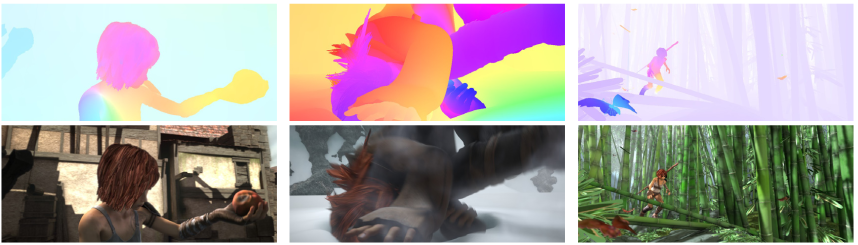
\includegraphics[width=0.8\linewidth]{../images/sintel_small.png}
\caption{ground truth flow (top), corresponding RGB-images (bottom)}
\end{figure}
\end{frame}

\begin{frame}
\frametitle{A naturalistic open source movie for optical flow evaluation}
\begin{itemize}
	\item dataset for optical flow estimation 
	\item derived from open source 3D animated short film \href{https://durian.blender.org/}{\textit{Sintel}}\\
	\item contains long sequences, large motions, specular reflections, motion blur, defocus blur, atmospheric effects and more
	\item authors use Blender to get ground truth optical flow maps
\end{itemize}
\end{frame}

\begin{frame}
\frametitle{Playing for data: Ground truth from computer games}
\cite{p4d}
\begin{figure}
	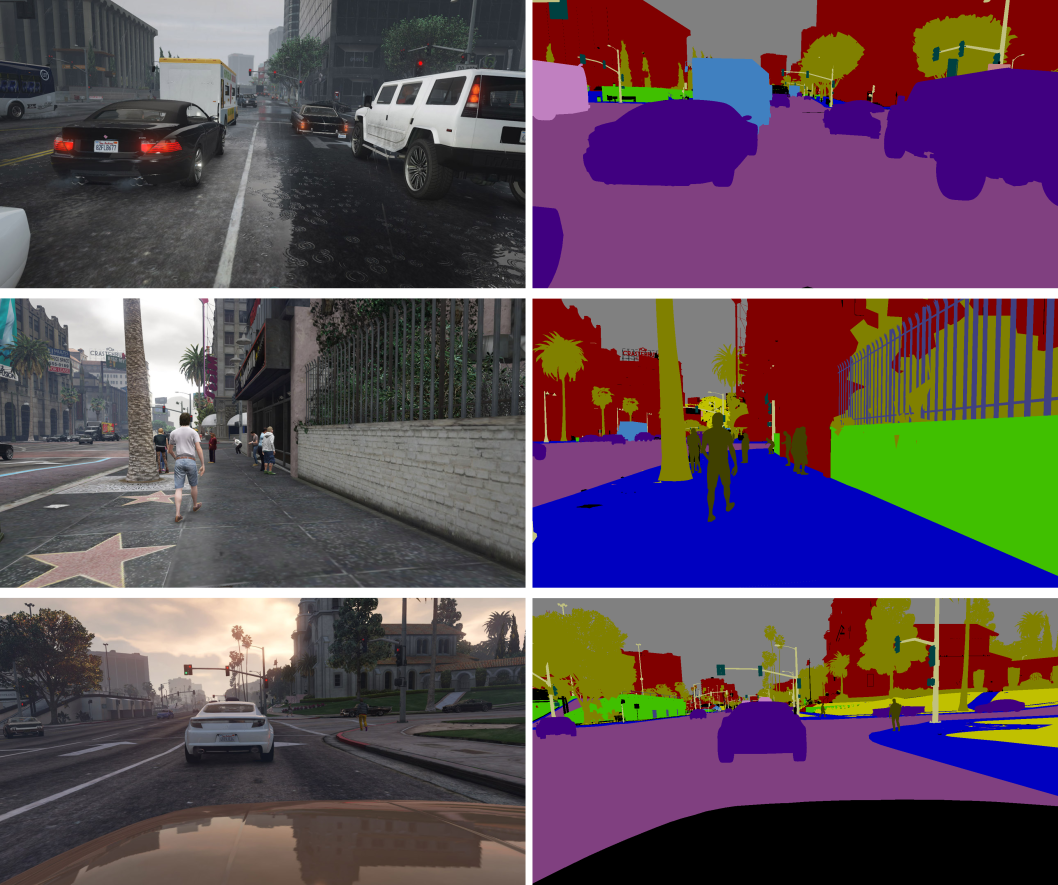
\includegraphics[width=0.5\linewidth]{../images/P4D.png}
	\caption{RGB images (left), corresponding semantic segmentation (right)}
\end{figure}
\end{frame}

\begin{frame}
\frametitle{Playing for data: Ground truth from computer games}

\begin{itemize}
	\item dataset containing RGB-images, depth-maps and pixel accurate semantic segmentation of frames from Grand Theft Auto V
	\item accomplished by saving rendering commands for geometry, textures, shaders from the game
	\item hash geometry, texture, shader to obtain object signatures
	\item while labeling, labels of objects get propagated to all frames containing the same object
\end{itemize}

\end{frame}

\begin{frame}
\frametitle{The SYNTHIA dataset: A large collection of synthetic images for semantic segmentation of urban scenes}
\cite{synthia}
\begin{columns}[c]
\column{.5\textwidth}
\begin{figure}
	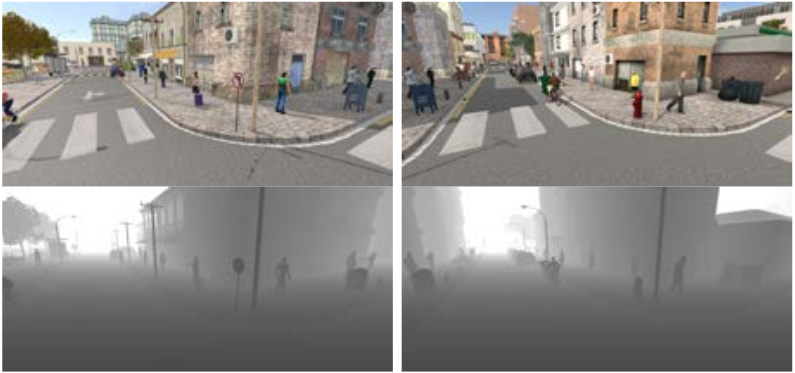
\includegraphics[width=\linewidth]{../images/SYNTHIA_depth_half.png}
	\caption{RGB images (top), corresponding depth-maps (bottom)}
\end{figure}
\column{.5\textwidth}
\begin{figure}
	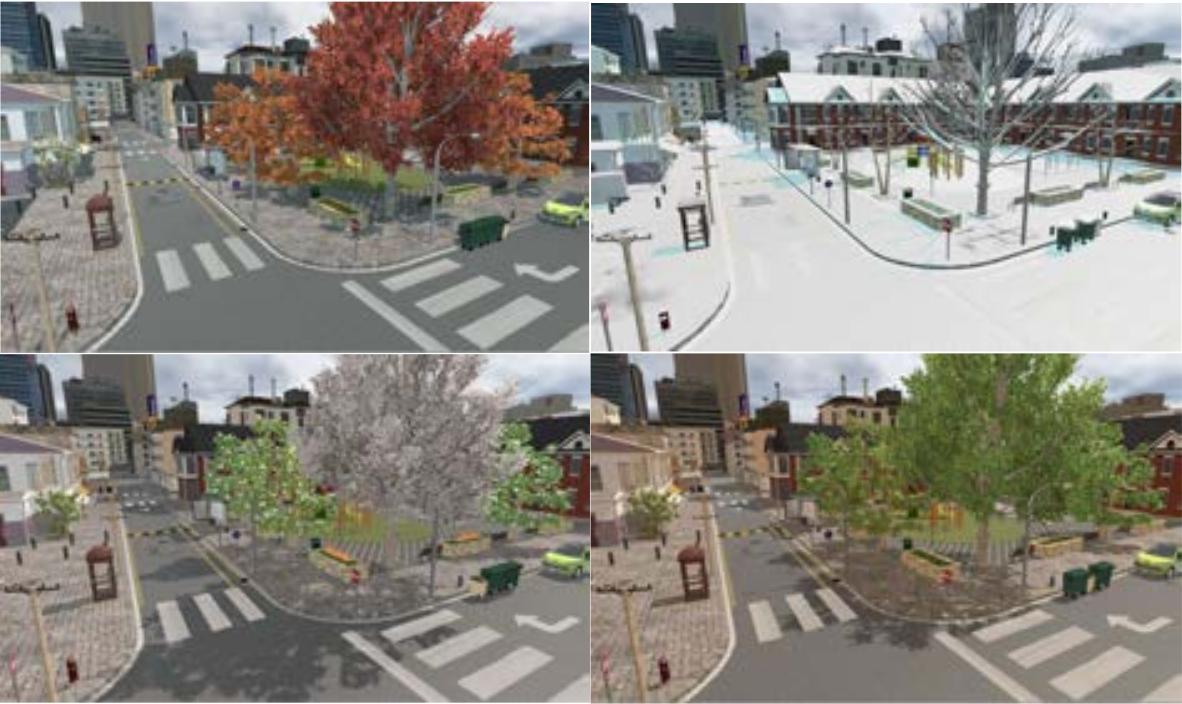
\includegraphics[width=\linewidth]{../images/SYNTHIA_seasons.png}
	\caption{from top left to bottom right: fall, winter, spring, summer}
\end{figure}
\end{columns}
\end{frame}

\begin{frame}
\frametitle{The SYNTHIA dataset: A large collection of synthetic images for semantic segmentation of urban scenes}

\begin{itemize}
	\item dataset containing RGB-images, depth-maps and pixel-level semantic segmentation of virtual city
	\item includes 4 different seasons (different weather conditions), day- and nighttime (varying lighting conditions)
	\item SYNTHIA-Rand: 13,400 frames of the city (camera randomly moved through city)
	\item SYNTHIA-Seq: one 50,000 frames video for each season (simulated car driving through city)
\end{itemize}

\end{frame}

\begin{frame}
\frametitle{SyB3R: A Realistic Synthetic Benchmark for 3D Reconstruction from Images}
\cite{syb3r}
\begin{figure}
	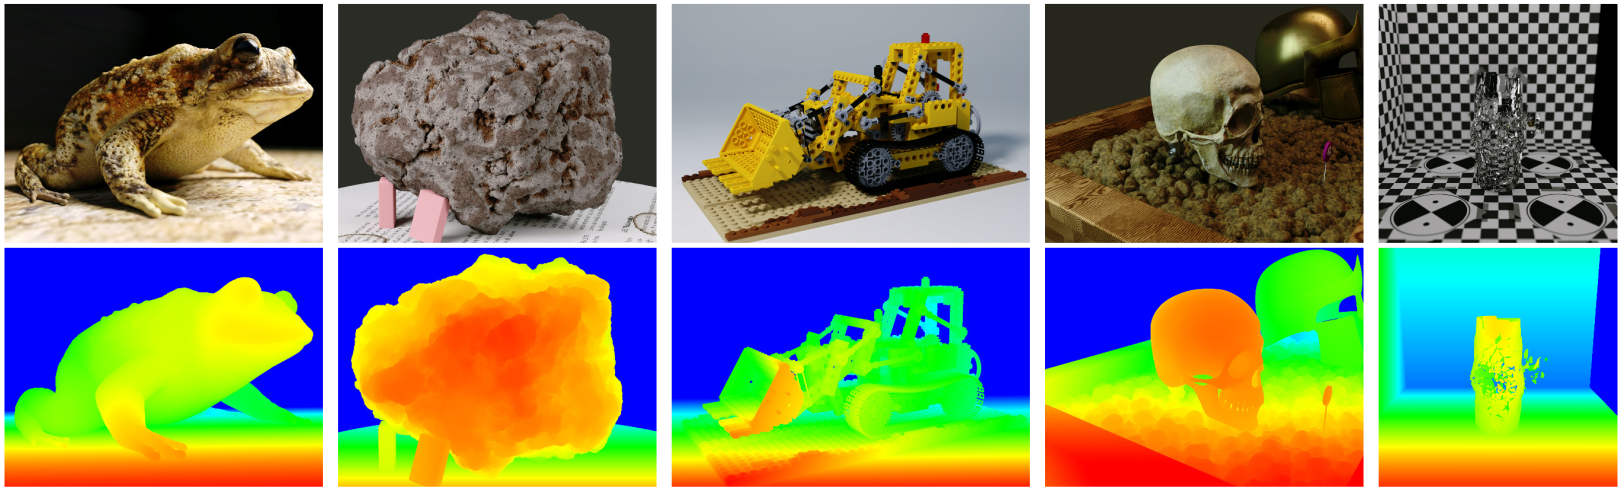
\includegraphics[width=\linewidth]{../images/SyB3R.png}
	\caption{RGB-images (top), depth-maps (bottom)}
\end{figure}
\end{frame}

\begin{frame}
\frametitle{SyB3R: A Realistic Synthetic Benchmark for 3D Reconstruction from Images}

\begin{itemize}
	\item framework to evaluate 3D reconstruction algorithms
	\item all camera parameters and 3D structure of scene is known
	\item includes real world effects like motion blur and noise
\end{itemize}
\begin{figure}
	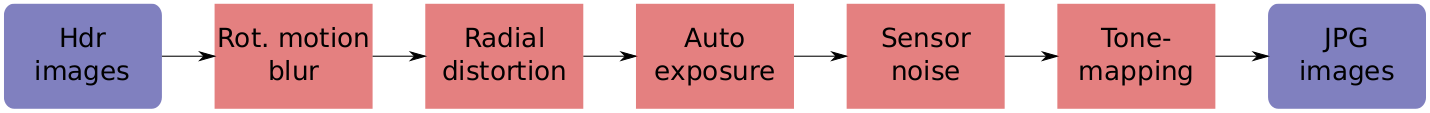
\includegraphics[width=\linewidth]{../images/SyB3R_pp.png}
	\caption{SyB3R's modular post processing pipeline}
\end{figure}

\end{frame}

\begin{frame}
	\frametitle{DeepMVS: Learning Multi-view Stereopsis}
	
\end{frame}

\subsection{Generative Adversarial Networks}

\begin{frame}
\frametitle{Image-to-Image Translation with Conditional Adversarial Networks}
\cite{i2i}
\begin{figure}
	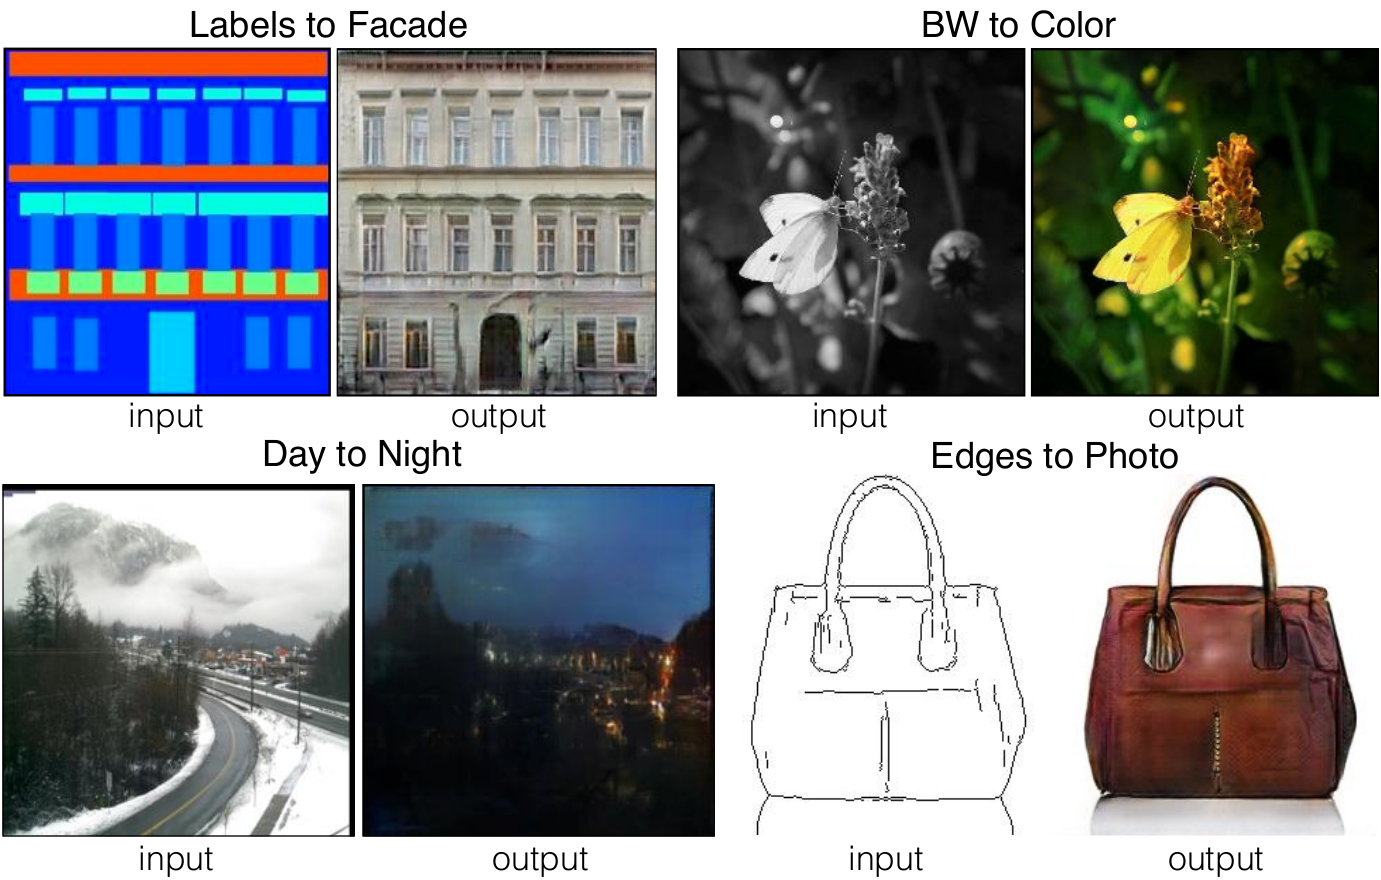
\includegraphics[width=0.6\linewidth]{../images/i2i.png}
	\caption{inputs and corresponding outputs to conditional GAN}
\end{figure}
\end{frame}

\begin{frame}
\frametitle{Image-to-Image Translation with Conditional Adversarial Networks}
\begin{figure}
	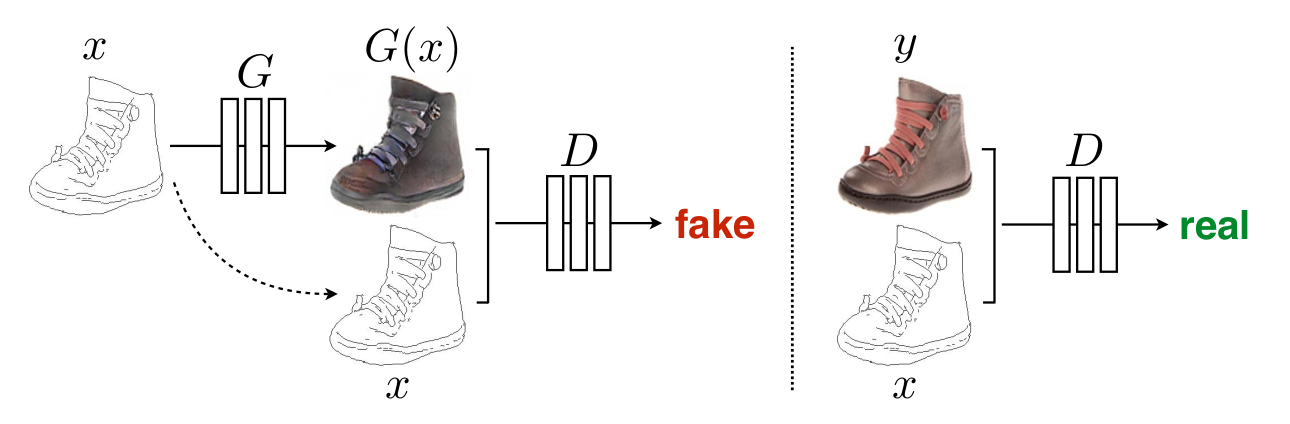
\includegraphics[width=\linewidth]{../images/i2i_GAN.png}
	\caption{schematic overview of how GANs work}
\end{figure}
\end{frame}

\begin{frame}
\frametitle{Image-to-Image Translation with Conditional Adversarial Networks}
\begin{figure}
	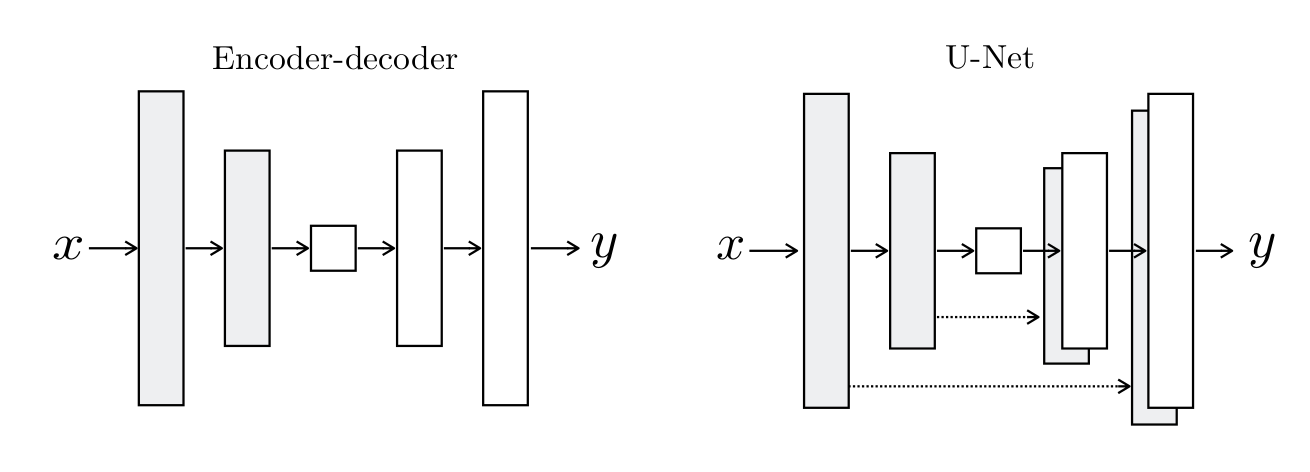
\includegraphics[width=\linewidth]{../images/i2i_unet.png}
	\caption{encoder-decoder and U-Net networks}
\end{figure}
\end{frame}

\begin{frame}
\frametitle{Image-to-Image Translation with Conditional Adversarial Networks}

\begin{itemize}
	\item TODO
\end{itemize}
\end{frame}

\begin{frame}
\frametitle{Unpaired Image-to-Image Translation	using Cycle-Consistent Adversarial Networks}
\cite{ui2i}
\begin{figure}
	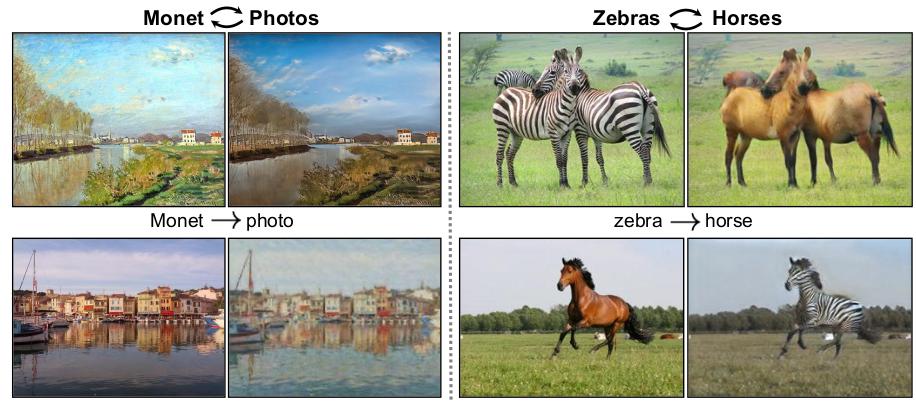
\includegraphics[width=0.9\linewidth]{../images/ui2i.png}
	\caption{images translated by cycleGAN}
\end{figure}
\end{frame}

\begin{frame}
\frametitle{Unpaired Image-to-Image Translation	using Cycle-Consistent Adversarial Networks}
\cite{ui2i}
\begin{figure}
	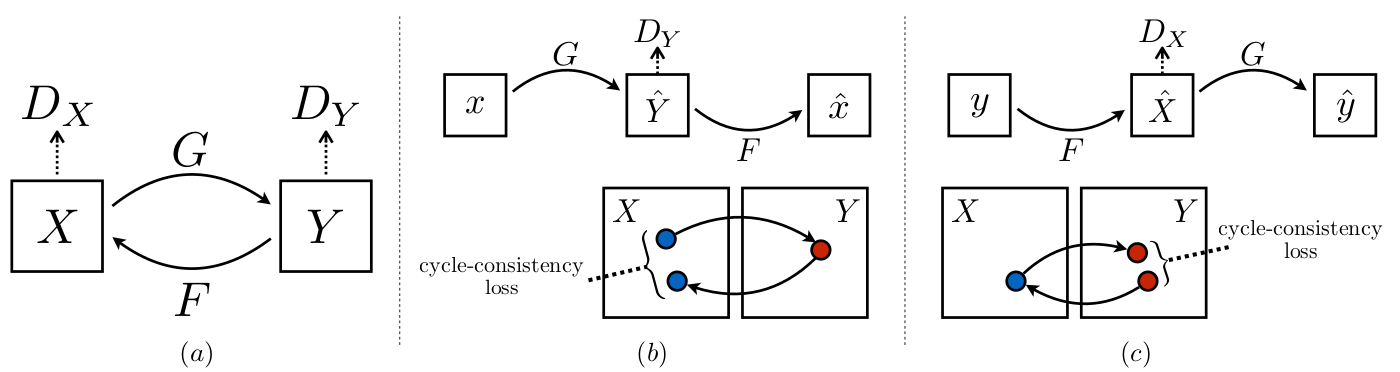
\includegraphics[width=\linewidth]{../images/ui2i_cycleGAN.png}
	\caption{schematic overview of full cycleGAN with domains X and Y, discriminators $D_X$ and $D_Y$ and Generators G and F}
\end{figure}
\end{frame}

\begin{frame}
\frametitle{Unpaired Image-to-Image Translation	using Cycle-Consistent Adversarial Networks}

\begin{itemize}
	\item TODO
\end{itemize}

\end{frame}

%\begin{frame}
%\frametitle{Image style transfer using convolutional neural networks}
%\cite{style}
%
%\begin{figure}
%	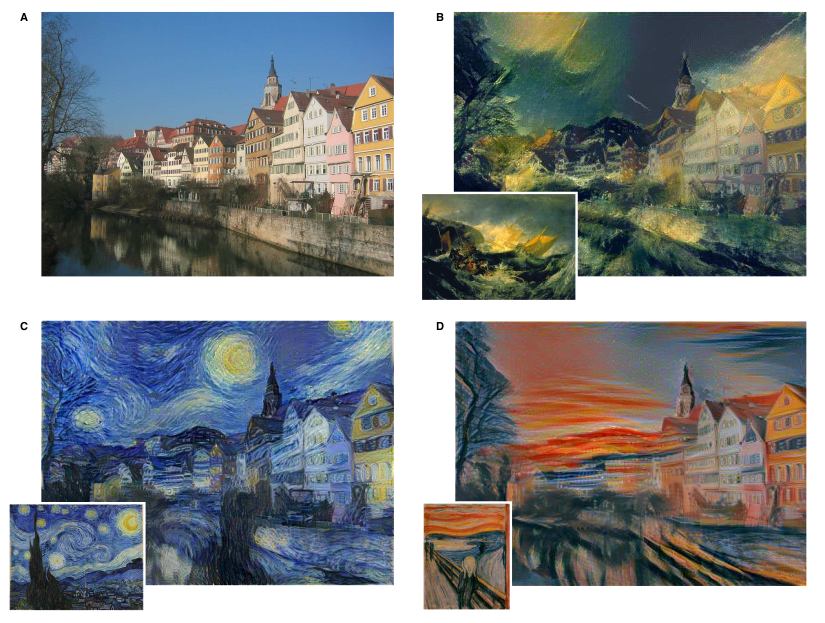
\includegraphics[width=0.55\linewidth]{../images/style.png}
%	\caption{top left: original image, others: result of transfering style of small images (each bottom left) to original image}
%\end{figure}
%
%\end{frame}
%
%\begin{frame}
%\frametitle{Image style transfer using convolutional neural networks}
%
%\begin{itemize}
%	\item TODO
%\end{itemize}
%
%\end{frame}

%------------------------------------------------
\section{Current Progress}
%------------------------------------------------

\subsection{dataset}

\begin{frame}
	\frametitle{RenderDoc}
	\begin{itemize}
		\item Website: \href{https://renderdoc.org/}{\textit{renderdoc.org}}
		\item graphics debugger
		\item allows single-frame capture with detailed introspection of applications using Vulkan, D3D11 and more
		\item free under \href{https://opensource.org/licenses/MIT}{\textit{MIT license}}
		\item used in playing-for-data and available at \href{https://bitbucket.org/visinf/projects-2016-playing-for-data}{https://bitbucket.org/visinf/projects-2016-playing-for-data/}
	\end{itemize}
\end{frame}

\begin{frame}
	\frametitle{Captures}
	\begin{figure}
		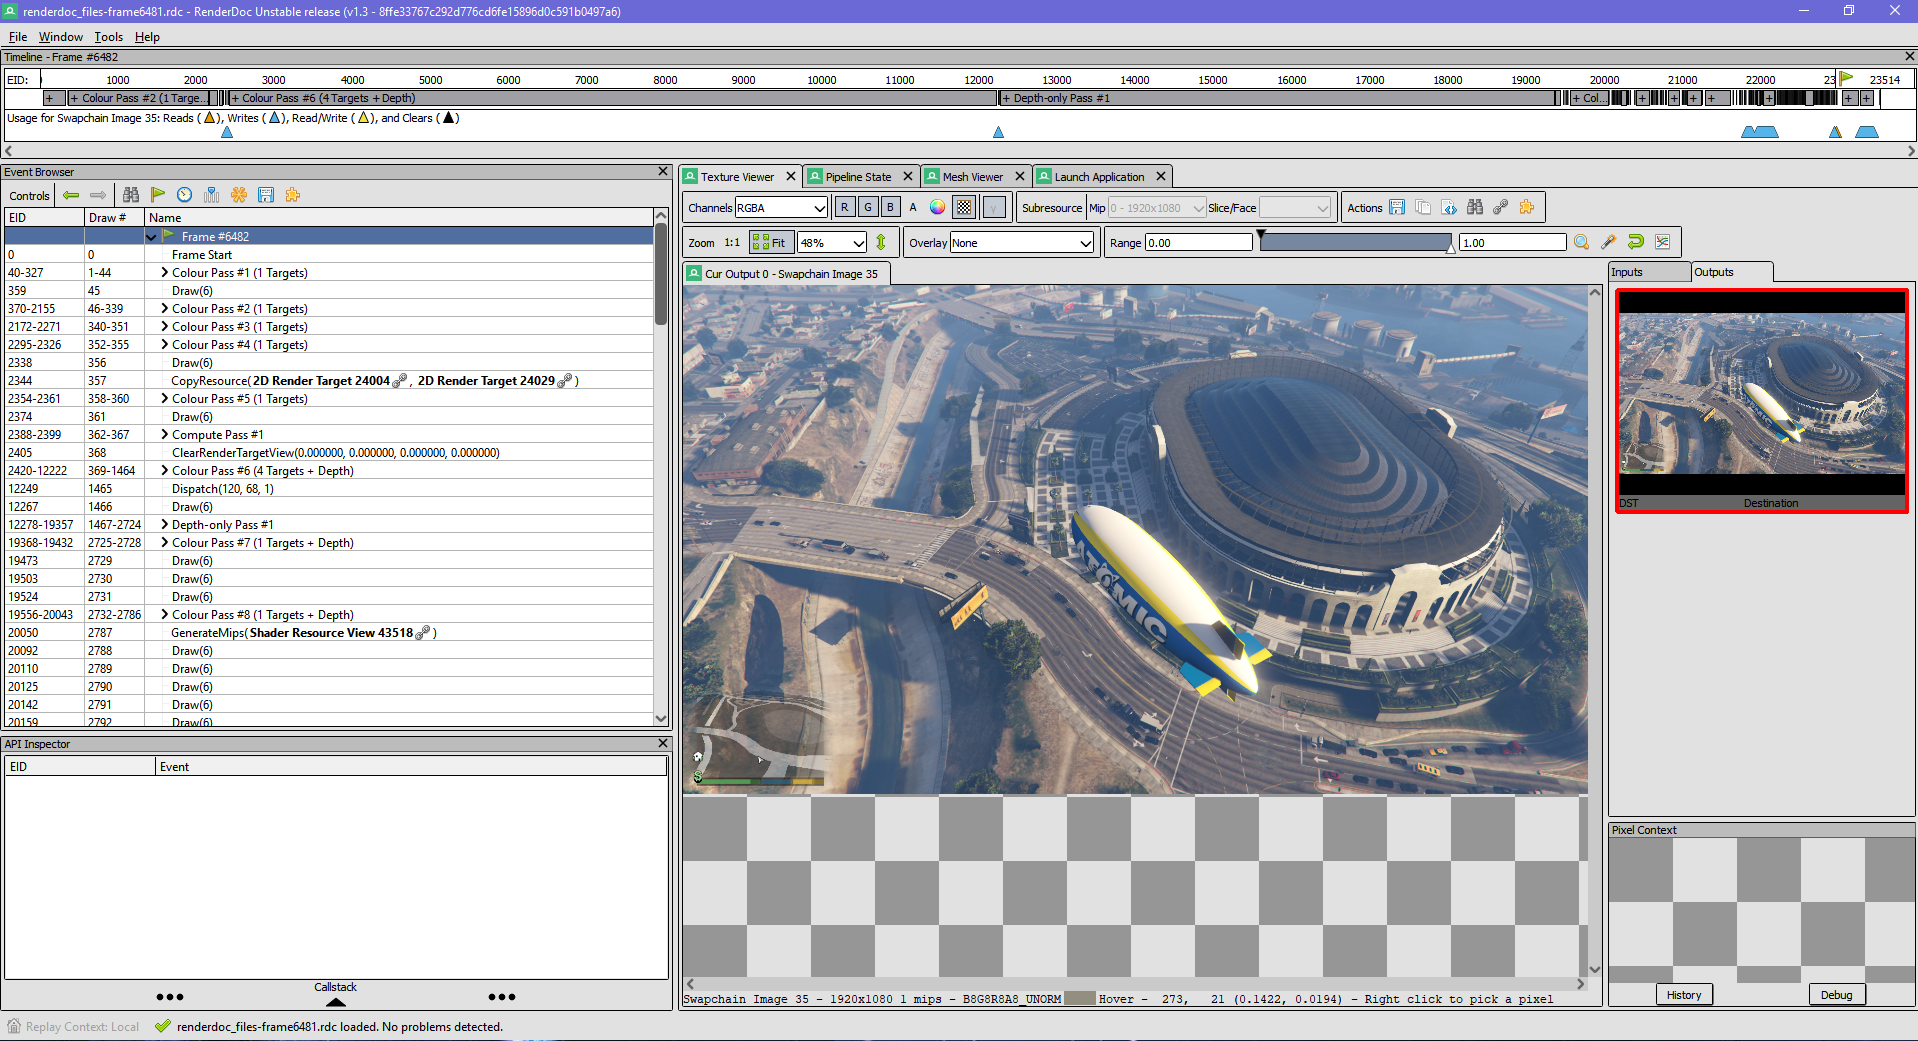
\includegraphics[width=0.9\linewidth]{../images/renderdoc.PNG}
		\caption{RenderDoc Capture from GTAV}
	\end{figure}
\end{frame}

\begin{frame}
	\frametitle{extract.py}
	\begin{itemize}
		\item python script to extract RGB-images, depth-maps and camera parameters
		\item original version available at \href{https://bitbucket.org/visinf/projects-2016-playing-for-data/}{\textit{https://bitbucket.org/visinf/projects-2016-playing-for-data/}}
		\item takes around 20-30 seconds per frame
	\end{itemize}
\end{frame}

\begin{frame}
	\frametitle{challenges}
	\begin{itemize}
		\item playing-for-data from 2016, due to GTAV updates their RenderDoc version can't capture anymore
		\item current RenderDoc version not compatible with extract.py
		\item playing-for-data RenderDoc included openEXR to save depth-maps, standard RenderDoc does not $\rightarrow$ depth-maps accuracy too low
		\item find the right drawcalls for depth-maps and RGB-images
	\end{itemize}
\end{frame}

\begin{frame}
	\frametitle{current state}
	\begin{itemize}
		\item modified RenderDoc to automatically capture every 40th frame ingame
		\item updated extract.py to work with current RenderDoc API
		\item not able to save depth-maps in high accuracy due to problems with dependencies while adding openEXR to current RenderDoc build
	\end{itemize}
\end{frame}

\begin{frame}
	\frametitle{looking forward}
	\begin{itemize}
		\item goal: finish thesis by end of July
		\item therefore: skip capturing frames (for now)
		\item use MVS-Synth dataset which also includes RGB-images, depth-maps and camera parameters from GTAV frames to train GANs
	\end{itemize}
\end{frame}


\subsection{GANs}


\section{References}

\begin{frame}
\frametitle{References}
\footnotesize{
\begin{thebibliography}{99} 
	\bibitem[Butler et. al]{sintel} Butler et al.
	\newblock A naturalistic open source movie for optical flow evaluation
	\newblock \emph{European Conf. on Computer Vision (ECCV)} Part IV, LNCS 7577, 611 -- 625. Springer-Verlag, October 2012
\end{thebibliography}

\begin{thebibliography}{99} 
	\bibitem[Ley et al.]{syb3r} Ley et al.
	\newblock
	\newblock \emph{SyB3R: A Realistic Synthetic Benchmark for 3D Reconstruction from Images}, pages 236 -- 251. Springer International Publishing, 2016
\end{thebibliography}

\begin{thebibliography}{99} 
	\bibitem[Ros et. al]{synthia} Ros et al.
	\newblock The SYNTHIA Dataset: A large collection of synthetic images for semantic segmentation of urban scenes
	\newblock 2016
\end{thebibliography}

\begin{thebibliography}{99} 
	\bibitem[Richter et. al]{p4d} Richter et al.
	\newblock Playing for data: Ground truth from computer games
	\newblock In Bastian Leibe et al., editors \emph{European Conf. on Computer Vision (ECCV)}, LNCS 9906, 102 -- 118. Springer International Publishing, 2016
\end{thebibliography}
}
\end{frame}



\begin{frame}
\frametitle{References}
\footnotesize{
	\begin{thebibliography}{99} 
		\bibitem[Huang et. al]{deepmvs} Huang et al.
		\newblock DeepMVS: Learning Multi-view Stereopsis
		\newblock \emph{CoRR}, abs/1804.00650, 2018
	\end{thebibliography}
	\begin{thebibliography}{99} 
		\bibitem[Isola et. al]{i2i} Isola et al.
		\newblock Image-to-image translation with conditional adversarial networks
		\newblock \emph{CoRR}, abs/1611.07004, 2016
	\end{thebibliography}

	\begin{thebibliography}{99} 
		\bibitem[Zhu et. al]{ui2i} Zhu et al.
		\newblock Unpaired image-to-image translation using cycle-consistent adversarial networks
		\newblock \emph{CoRR}, abs/1703.10593, 2017
	\end{thebibliography}
}
\end{frame}
%------------------------------------------------

\begin{frame}
\titlepage
\end{frame}

%----------------------------------------------------------------------------------------

\end{document} 